\section{Konkurrenzanalyse}\label{sec:konkurrenzanalyse}
Diese Arbeit beginnt mit einer Konkurrenzanalyse der Webseiten www.google.com, www.bing.com sowie www.qwant.com.
Dabei wird insbesondere auf den Inhalt der jeweiligen Webseiten, die Zielgruppenorientierung, das Design, die Informations-
und Navigationsarchitektur, die Texte sowie auf die Technik der Seiten eingegangen.
Zusätzlich zu diesen Punkten wird auch auf die Qualität der Suchvorschläge eingegangen.

\subsection{Inhalt}\label{subsec:inhalt}
Das Ziel aller drei Webseiten ist es, den Nutzern die Möglichkeit zu bieten, das Internet nach Webseiten zu einem gewissen
Thema zu durchsuchen.
Ohne das Vorwissen, dass die drei Seiten dies anbieten, ist diese Dienstleistung allerdings nicht auf den ersten
Blick erkenntlich.
\begin{figure}[ht]
    \centering
    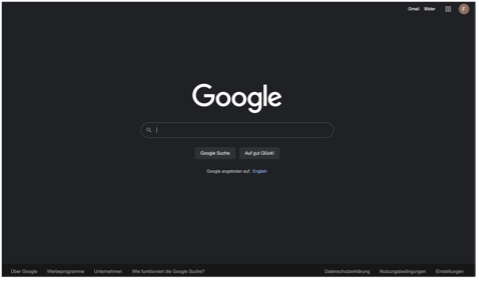
\includegraphics{Google Startseite}
    \caption{Startseite von Google}\label{fig:figure}
\end{figure}

Beispielsweise besteht die Startseite von Google nur aus einer Leiste, in der man etwas eingeben kann.
Ohne eine Anleitung, was sie in dieser Leiste eingeben können, führt dies am Anfang für Verwirrung.
Nutzer, die mit Google vertraut sind, profitieren allerdings von dieser Anordnung, da diese nicht von der Funktionalität ablenkt.
\begin{figure}[ht]
    \centering
    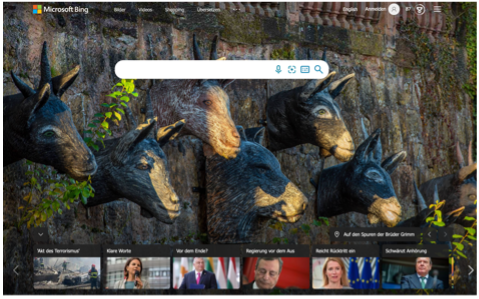
\includegraphics{Bing Startseite}
    \caption{Startseite von Bing}\label{fig:figure2}
\end{figure}
Einen ähnlichen
Aufbau bietet Microsoft mit ihrer Suchmaschine Bing.
Hierbei werden standardmäßig allerdings noch aktuelle Nachrichten sowie ein Hintergrundbild angezeigt.
\begin{figure}[ht]
    \centering
    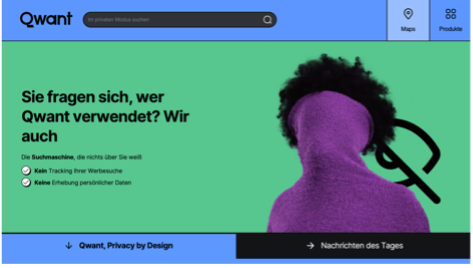
\includegraphics{Qwant Startseite}
    \caption{Startseite von Qwant}\label{fig:figure3}
\end{figure}
Einzig Qwant folgt diesem Schema nicht ganz.
Bei dieser Seite ist die Suchleiste, welche die
Hauptfunktion ist, im oberen Bereich, wodurch der Fokus auch auf die Texte in der Mitte des Bildschirms fallen kann.
Dies erschwert es Erstanwendern noch mehr als bei den Konkurrenten, die Funktion intuitiv zu bedienen.
Somit mangelt es allen Suchmaschinen an Selbstbeschreibungsfähigkeit.
Dies wäre nur gewährleistet, \gqq{wenn jeder einzelne Dialogschritt unmittelbar verständlich ist.}\autocite[Seite 6]{Maulhardt2}
Auch adäquate Anleitungen werden nicht zur Verfügung gestellt.

Trotz der oben genannten Kritik bieten alle drei Suchmaschinen, insbesondere für erfahrene Anwender, einen echten Mehrwert.
So erleichtern es alle Seiten, sich im Internet zurechtzufinden und ermöglichen das Finden bestimmter Webseiten.

\subsection{Zielgruppenorientierung}\label{subsec:zielgruppenorientierung}
Wie jedes Produkt haben auch diese drei Webseiten Zielgruppen, welche durch verschiedene Aspekte wie Design oder Inhalt
angesprochen werden sollen.
Diese Zielgruppen sollen nachfolgend herausgearbeitet werden und die Orientierung an diesen
bewertet werden.

Um herauszufinden, wie gut die drei Seiten ihre Zielgruppen abbilden, ist es zuerst nötig, diese Zielgruppen zu identifizieren.
Diese Adressaten haben bei allen drei Seiten eine große Schnittmenge, unterscheiden sich allerdings in Kleinigkeiten.
Da alle drei Unternehmen, welche die Suchmaschinen betreiben, einen möglichst großen Umsatz durch Werbeplatzierungen
erzielen wollen, versuchen diese, eine möglichst große Zahl an Usern zu generieren, weswegen die Seiten auch auf diesen Zweck zugeschnitten sind.
Da nicht alle Menschen Zugang zu Internet haben, richten sich die Webseiten, insbesondere an Personen mit diesem Zugang.
Ansonsten ist die Bandbreite an potenziellen Nutzergruppen sehr groß.
Dies erkennt man auch an der großen Auswahl an Sprachen, in welchen die Webseiten dargestellt werden können.
So bietet Google knapp 150 Sprachen an, Bing knapp 100.
Qwant müsste sich hingegen noch breiter aufstellen.
Mit gerade einmal 12 Sprachen wird eine große Zahl an
potenziellen Nutzern nicht angesprochen.

Eine Besonderheit gibt es bei der Zielgruppe von Qwant jedoch noch zu beachten.
Sie versuchen vornehmlich Leute anzusprechen, denen Privatsphäre wichtig ist.
Dies wird bereits auf der Startseite klar.
Auf dieser wird damit geworben, dass die Suchmaschine
nichts über die Nutzer weiß, da diese keine persönlichen Daten erheben oder die Websuche tracken.

Ebenfalls spricht die Suchmaschine Qwant eine kindlichere Zielgruppe bzw.\ deren Eltern an.
In einem klar abgegrenzten Bereich wird es den Eltern ermöglicht, für die Kinder eine sichere Suche im Internet zu gewährleisten.
Bei den Konkurrenten fehlt ein solches Angebot.

\subsection{Design}\label{subsec:design}
Ein wichtiger Punkt einer Webseite ist dessen Design.
\gqq{Unser visuelles System ist darauf ausgelegt, schnell zu entscheiden, ob wir etwas gut oder schlecht finden.
Dabei wird der Ersteindruck einer Website vor allem durch die Schönheit,
    also die visuelle Ästhetik, bestimmt.}\autocite[Seite 43]{Thielsch2}
Somit ist das Design eines der zentralen Elemente, welches besonders gut ausgearbeitet sein muss.
Dabei gehen alle drei Suchmaschinen einen anderen Weg.

Googles Auftritt ist sehr minimalistisch gehalten.
Bis auf ein Logo, welches sich in unregelmäßigen Zeitabständen verändert,
ist nur die Suchleiste in der Bildmitte zu sehen.
Der Hintergrund ist dabei je nach Einstellung des Dark-Modes dunkelgrau oder weiß.
Diese fehlende Farbauswahl spiegelt nicht direkt das Firmenimage von Google wider, welches, wie am farbenfrohen
Firmenlogo zu erkennen, eher verspielt, modern und innovativ wirkt.
\begin{figure}[ht]
    \centering
    
\includegraphics[width=0.3\linewidth]{Google Firmenlogo}
    \caption{Firmenlogo von Google\autocite{GoogleLogo}}\label{fig:figure4}
\end{figure}

Im Gegensatz zu diesem einfarbigen Design von Google bietet Bing die Möglichkeit ein Landschaftsbild, als Hintergrund zu
setzen, welches sich täglich ändert.
Diese Veränderung bringt regelmäßige Abwechslung, was auf den Nutzer erfrischend wirken kann.
Außerdem wirken die Bilder freundlich auf die Nutzer, weswegen die Startseite von Bing, gegenüber der von Google,
bevorzugt werden könnte.
\begin{figure}[ht]
    \centering
    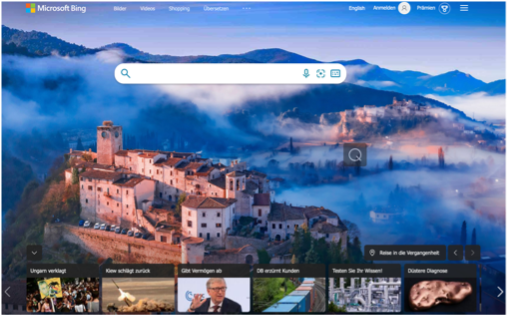
\includegraphics{Bing Startseite 2}
    \caption{Design der Startseite von Bing}\label{fig:figure5}
\end{figure}

Am auffälligsten und damit auch am meisten Raum für Analyse bietend ist allerdings die Startseite von Qwant.
Mehrere klassische Formen des Kontrasts wurden hier benutzt.
Zum einen ist der starke Kontrast zwischen gelb und blau auffällig.
\begin{figure}[ht]
    \centering
    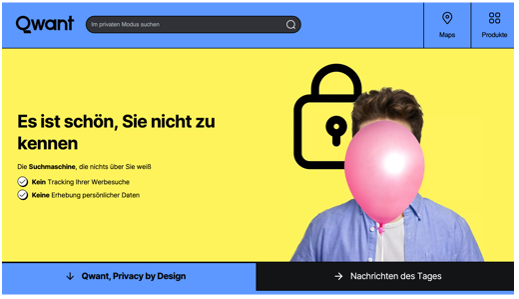
\includegraphics{Qwant Startseite Design}
    \caption{Design der Startseite von Qwant}\label{fig:figure6}
\end{figure}
Dies erinnert stark an einen Komplementärkontrast.
Dies bedeutet, dass sich die beiden Farben im Farbenkreis gegenüberliegen.\autocite[Seite 33]{Maulhardt3}
Bei Betrachtung des Farbkreises nach Itten (\ref{fig:farbkreis}) fällt dies ebenfalls auf.
Auch ein Warm-Kalt-Kontrast ist vorhanden.
Hierbei wird die warme Farbe Gelb der kalten Farbe Blau direkt gegenübergestellt.\autocite[Seite 34]{Maulhardt3}
Zuletzt beinhaltet die Startseite noch einen Farbe-an-sich-Kontrast.
\begin{figure}[ht]
    \centering
    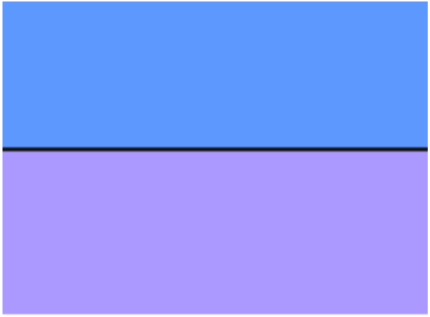
\includegraphics{Qwant Startseite 3}
    \caption{Startseite von Qwant}
    \label{fig:qwantstartseite3}
\end{figure}
Dieser ergibt sich dadurch,
dass wie bei Abbildung~\ref{fig:qwantstartseite3} die Grundfarben Blau und Lila gegenübergestellt werden.\autocite[Seite 38]{Maulhardt3}
All diese Kontraste lassen die Startseite von Qwant lebendig wirken, was mit dem Image der Firma bzw.\ der Suchmaschine übereinstimmt.
Trotzdem wäre es wünschenswert, wenn das Erscheinungsbild angepasst werden könnte, da dies einigen aufgrund der starken
Kontraste abschrecken könnte.
Diese junge Zielgruppe ist auch aufgrund der Benutzung von Emojis in beispielsweise den
Filtereinstellungen erkennbar.

Positiv fällt bei allen drei Seiten auf, dass diese einen einstellbaren Dark Mode besitzen, welcher es ermöglicht, das Design zu verändern.
Zusätzlich bietet Bing die Möglichkeit das oben angesprochene Hintergrundbild nicht anzeigen zu lassen,
sodass die Optik mit entweder dunkelgrau oder weiß als Hintergrund sehr stark Google ähnelt.

\subsection{Informations- und Navigationsarchitektur}\label{subsec:informations--und-navigationsarchitektur}
Die Navigationsarchitektur ist auf allen drei Seiten relativ gleich aufgebaut.
Die Startseite besteht dabei aus einer Suchleiste,
welche nach der Suche an den oberen Bildrand geht, wobei die vorgeschlagenen Webseiten darunter angezeigt werden.
Das Logo der Suchmaschine dient dabei immer als Home button.
Diese Grundstruktur ist für Personen, die die Funktionalität der
Seiten kennen sehr einfach zu durchschauen, da sie sich von Anbieter zu Anbieter nicht verändert.
Allerdings unterscheidet sich die Architektur in Kleinigkeiten.
Darauf wird im Nachfolgenden eingegangen.

Google bietet in der rechten oberen Ecke die Möglichkeit, den Account zu managen, auf zahlreiche andere Google Dienste zu
wechseln oder eine Bilder-Suche durchzuführen.
Am unteren Bildrand wird zum einen auf Informationsseiten zu Google verwiesen,
wie auch die Möglichkeiten geboten, die Einstellungen zu ändern.
Diese Auswahlmöglichkeiten sind allerdings sehr klein gehalten,
wodurch sie für Leute, welche nicht mehr so gut sehen können, nicht mehr gut erkennbar sind.
Auch ein geringer Kontrast erschwert die Lesbarkeit dieser Elemente.

Bing hat im Gegensatz zu Google ein paar Punkte, welche positiv aufgefallen sind.
Insbesondere die Möglichkeit, sich Newsartikel sich anzeigen zu lassen,
auf welche man bei Bedarf klicken kann, stach dabei im direkten Vergleich heraus.
Ein weiterer Punkt ist die Verwendung von Icons, welche bei Google nur sehr wenig eingesetzt werden.
Dahingegen schafft es Bing, diese gezielt und unterstützend zu normalem Test einzusetzen, was die Bedienung vereinfacht.
\begin{figure}[ht]
    \centering
    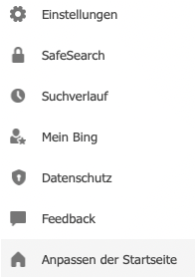
\includegraphics{Bing Icons 1}
    \caption{Icons von Bing}\label{fig:figure8}
\end{figure}
Diese Icons sind dabei auch gemäß den Regeln
für die Gestaltung einer Navigationsleiste\autocite[Seite 17]{Maulhardt6} selbsterklärend, da sie alle standardmäßig auch von
anderen Webseiten für dieselben Funktionen verwendet werden.

Zuletzt wird die Navigationsstruktur von Qwant analysiert.
Diese hat sowohl Vor- als auch Nachteile gegenüber den Konkurrenten.
Zum einen ist die Zahl an Auswahlpunkten, zumindest wenn auf der Startseite nicht gescrollt wird, sehr leicht überschaubar.
So kann man nur zwischen Maps, den Produkten, Informationen über Qwant und den Nachrichten des Tages wählen.
Diese geringe Zahl ermöglicht es, vor allem im Vergleich zu den Konkurrenten,
welche 13 (Google) und 9 (Bing) Auswahlpunkte direkt auf der
Startseite haben, schnell einen Überblick über die Struktur der Seite zu erlangen.
Damit halten sich die beiden Seiten auch nicht an die Regel,
dass nur maximal sieben Buttons gleichzeitig zu sehen sind, da das Gehirn nicht mehr auf einen Blick
wahrnehmen kann.\autocite[Seite 16]{Maulhardt6}
Negativ wiederum an der Startseite von Qwant ist, dass der Punkt „Maps“, welcher
in Abbildung~\ref{fig:qwantnavigation} zu sehen ist, sich mit dem Menü, welches unter Produkte gezeigt wird, überschneidet.
\begin{figure}[ht]
    \centering
    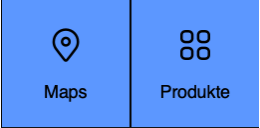
\includegraphics{Qwant Navigation}
    \caption{Navigation von Qwant}
    \label{fig:qwantnavigation}
\end{figure}

So werden dabei die
Produkte Search und Maps vorgeschlagen, obwohl man auf Search bereits ist und Maps einfacher über den extra Button Maps aufrufbar ist.
Einzig das Produkt „Junior“ ist in dieser Reihe neu.
Ebenso negativ anzumerken ist, dass die Einstellungen schwer zu finden sind.
So muss der Nutzer bis ganz nach unten scrollen, damit sehr klein unten rechts der Button Einstellungen zu sehen ist.
Dieser ist zusätzlich nicht einmal deutlich hervorgehoben und wird mit grauer Schrift auf schwarzem Hintergrund dargestellt.

\subsection{Text}\label{subsec:text}
Aufgrund der Ziele der Webseitenbetreiber sind die Seiten mit wenig Text versehen.
Stattdessen ist der Aufbau der Seiten so gestaltet, dass der Nutzer sich intuitiv zurechtfindet.
Außerdem ist es nicht das Ziel der Suchmaschinen den User durch lange Texte vom eigentlichen Sinn der Seite abzulenken,
nämlich dem Suchen nach anderen Webseiten.
Einzig Qwant fällt aus diesem Muster heraus.
\begin{figure}[ht]
    \centering
    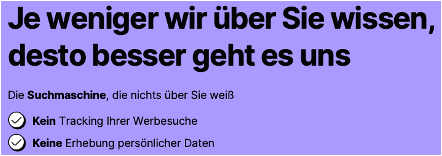
\includegraphics{Qwant Texte}
    \caption{Texte von Qwant}\label{fig:figure9}
\end{figure}

Sie versuchen den Besucher auf der Homepage von ihrem Konzept der privaten Suche mit der Hilfe von Text zu überzeugen.
Dabei befolgen Sie auch alle Regeln der Textgestaltung\autocite[Seite 5ff]{Maulhardt6}.
Durch kurze prägnante Texte, in welchen durch fette Schrift das wichtigste markiert ist, wird die Kernaussage gut dargestellt.

\subsection{Technik}\label{subsec:technik}
Ebenso wichtig wie die bisher angesprochenen Analysekriterien ist die Technik, mit welcher die Webseiten gestaltet wurden.
So können beispielsweise lange Ladezeiten dafür sorgen, dass der Nutzer eine andere Suchmaschine in Zukunft benutzen wird.
Um diese Technik möglichst objektiv bewerten zu können wurde ein standardisierter Test durchgeführt,
welcher Webseiten nach vier Analysekriterien beurteilt.
Dieser Test namens „Lighthouse“ ist dabei eine Chrome-Erweiterung.
Die genauen Ergebnisse sind im Anhang zu finden.

Google schneidet dabei am besten ab.
Nur im Bereich SEO, was für Search Engine Optimization steht, ist noch wirkliches
Potenzial, die Seite zu verbessern.
Ansonsten ist Google in den drei Bereichen Performance Accessibility und Best Practices in einem sehr guten Bereich.
Insbesondere die Performance, welche bei den anderen beiden Anbietern schlechter ist, sticht dabei heraus.

Bing hingegen hat vornehmlich im Bereich Performance noch Verbesserungsbedarf.
Hierbei wird empfohlen, ungenutzten JavaScript Code zu reduzieren.
Ebenso könnte der Analysepunkt Accessibility besser sein.

Qwant schneidet im Bereich Performance mit gerade einmal 54 von 100 möglichen Punkten am schlechtesten ab.
Dabei wird ebenfalls geraten, ungenutzten JavaScript Code zu reduzieren.

\subsection{Qualität der Suchvorschläge}\label{subsec:qualitat-der-suchvorschlage}
Bei der Analyse einer Suchmaschine sind auch die Suchvorschläge sowie die Ergebnisse zu evaluieren.
Dies wurde exemplarisch an dem Begriff Medientechnik untersucht.
Google und Bing sind dabei auf einem vergleichbaren Niveau.
Beide Suchmaschinen bieten zahlreiche Möglichkeiten zum bisher eingegebenen Begriff \gqq{Mediente} ,
wie beispielsweise „Medientechnik“ oder \gqq{Medientechnologe} .

Ebenso werden zahlreiche verschiedene Informationen nach der Suche präsentiert,
welche über die reine Auflistung von Webseiten hinausgehen.
So boten beide Webseiten Unternehmen in der Nähe des Benutzers an.
Bing präsentierte zusätzlich Videos,
wohingegen Google auf den Wikipedia Artikel zu Medientechnik verwies.

Dahingegen bot Qwant keine Vervollständigung des Begriffs \gqq{Mediente} an.
Ebenso besteht Verbesserungsbedarf in der Präsentation der Webseiten.
In diesem Fall wurden nur mögliche Webseiten aufgelistet,
während beispielsweise Google interaktive Schaltflächen zu Maps und Wikipedia anbot.